%HEADER
\documentclass[12pt,letterpaper]{article}

%packages
\usepackage{fixltx2e}
\usepackage{textcomp}
\usepackage{fullpage}
\usepackage{amsfonts}
\usepackage{verbatim}
\usepackage[english]{babel}
\usepackage{pifont}
\usepackage{color}
\usepackage{setspace}
\usepackage{lscape}
\usepackage{indentfirst}
\usepackage[normalem]{ulem}
\usepackage{booktabs}
%\usepackage{nag}
\usepackage{natbib}
%\usepackage{bibtex}
\usepackage{float}
\usepackage{latexsym}
%\usepackage{hyperref} 
\usepackage{url}
%\usepackage{html}
\usepackage{hyperref}
\usepackage{epsfig}
\usepackage{graphicx}
\usepackage{amssymb}
\usepackage{amsmath}
\usepackage{bm}
\usepackage{array}
\usepackage[version=3]{mhchem}
\usepackage{ifthen}
\usepackage{caption}
\usepackage{hyperref}
%\usepackage{xcolor}
\usepackage{amsthm}
\usepackage{amstext} % Add and remove packages as necessary for your manuscript.

%Pagination style and stuff
\linespread{1.66} % All text should be double-spaced with occasional exceptions for tables. 
\raggedright
\setlength{\parindent}{0.5in}

\setcounter{secnumdepth}{0} % Our sections are not numbered and our papers do not have Tables of Contents. We don't present a list of figures or list of tables, either. Any common font is fine. (A common sans-serif font should be used on figures, but figures should be separate from the LaTeX document.)

\pagestyle{empty}

\renewcommand{\section}[1]{%
\bigskip
\begin{center}
\begin{Large}
\normalfont\scshape #1
\medskip
\end{Large}
\end{center}}

\renewcommand{\subsection}[1]{%
\bigskip
\begin{center}
\begin{large}
\normalfont\itshape #1
\end{large}
\end{center}}

\renewcommand{\subsubsection}[1]{%
\vspace{2ex}
\noindent
\textit{#1.}---}

\renewcommand{\tableofcontents}{}

\bibpunct{(}{)}{;}{a}{}{,}  % this is a citation format command for natbib

%START
\begin{document}

%Runing head
\begin{flushright}
Version dated: \today
\end{flushright}
\bigskip
\noindent RH: Missing data in Total Evidence Supermatrices %RH = Running Head

\bigskip
\medskip
\begin{center}

%Title
\noindent{\Large \bf Effect of missing data in supermatrices containing living and fossil taxa on topological accuracy}
\bigskip

% We don't use a special title page; the author information is entered like any other text.
% FOOTNOTES: We don't allow them in the manuscript, except in tables. Don't include any footnotes in the text.

%Authors
\noindent {\normalsize \sc Thomas Guillerme$^1$$^,$$^2$, other authors $^3$, and Natalie Cooper$^1$$^,$$^2$}\\
\noindent {\small \it 
$^1$School of Natural Sciences, Trinity College Dublin, Dublin 2, Republic of Ireland;\\
$^2$Trinity Centre for Biodiversity Research, Trinity College Dublin, Dublin 2, Republic of Ireland;\\
$^3$Somewhere else }\\
\end{center}
\medskip
\noindent{\bf Corresponding author:} Thomas Guillerme, School of Natural Sciences, Trinity College Dublin, Dublin 2, Republic of Ireland; E-mail: guillert@tcd.ie.\\
\vspace{1in}


%Abstract
\subsubsection{Abstract}
Living species represent less than 1\% of all species that have ever lived. Ignoring fossil taxa may lead to misinterpretation of macroevolutionary patterns and processes such as trends in species richness, biogeographical history or paleoecology. This fact has led to an increasing consensus among scientists that both fossil and living taxa must be included in macroevolutionary studies. One approach, the Total Evidence Method, uses molecular data from living taxa and morphological data from both living and fossil taxa to infer phylogenies with both fossil and living taxa at the tips. Although the Total Evidence Method seems very promising, it requires a lot of data and is therefore likely to suffer from missing data issues which may affect its ability to infer correct phylogenies.

In this study we assess the effect of missing data on tree topologies inferred from total evidence supermatrices. Using simulations we investigate three major factors that directly affect the completeness of the morphological part of the supermatrix: (1) the proportion of living taxa with no morphological data, (2) the amount of missing data in the fossil record and (3) the overall number of morphological characters in the supermatrix. We find that, in a Bayesian framework, difficulties in recovering a stable topology are mainly driven by the missing data in the molecular part of the matrix (for which fossil taxa have no data). In a Maximum Likelihood framework, however, topology is not directly affected by missing data \textit{per se}, but by the number of morphological characters shared among the taxa. Therefore, the two main drivers of incorrect topologies are the overall number of morphological characters and the number of living species with no morphological data.

Our results suggest that, in order to use total evidence methods, one should reduce the missing data in the morphological part of the supermatrix for living species and use a Maximum Likelihood framework to fix the topology prior to the overall Bayesian phylogenetic inference process. We apply our method to a comprehensive data set of both living and fossil primates. We find that using this integrative method modifies previous estimates of rates of body mass evolution within primates.

\noindent (Keywords: bla, bla, bla)\\

\vspace{1.5in}

\newpage 

%We don't use a heading for the introduction. The nature of this section is implied by its position following the abstract and preceding the first major section heading.
Living species represent less than 1\% of all species that have ever lived \citep{novacek1992ext,raup1993extinction}. However, the majority of macroevolutionary studies focus solely on living species \citep{cooperwhat2009,meredithimpacts2011}.
Ignoring fossil taxa may lead to misinterpretation of macroevolutionary patterns and processes such as species richness gradients, e.g. extant clade diversity may ignore past diversification patterns \citep{shoshani1996proboscidea}; biogeographical history, e.g. extant biogeographical patterns are improved when integrating fossil data \citep{metcalfintegrating2014}; or paleoecology, e.g. extant clades niches might have differed greatly through time \citep{youngthe2010}. %Rewrite that part
These factors have led to increasing consensus among scientists that fossil taxa must be included in macroevolutionary studies \citep{jacksonwhat2006,quentaldiversity2010,dietlconservation2011,slaterunifying2013,fritzdiversity2013}. However, to do this we need to be able to place living and fossil taxa into the same phylogenies which still remains complex.

Three main approaches have been used for combining fossil and living taxa data in phylogenies. These approaches differ in whether they treat fossil taxa as nodes or tips and how much of the available data is used (i.e. age only or age and morphology). Classical cladistic methods use morphological data from both fossil and living taxa and treat each taxon as a tip \citep{simpson1945}. This approach is commonly used by paleontologists but it ignores
the majority of %You proposed to remove that. The point here was to not get in trouble with modern paleontologist that feel "clever" using DNA as a binary character like "Presence/absence of this SINE/that microsatellite"…
the additional molecular data available from living species. Neontologists, on the other hand, more commonly use only molecular data from living species to build phylogenies. Because fossil taxa do not usually have available DNA, fossils are used as nodes rather than tips in these analyses and only their occurrence age is used to time calibrate phylogenies \citep{zuckerkandl1965}. There have been great improvements in the theory and application of these two approaches \citep[e.g.][]{bapsta2013,stadlerdating2013,heaththe2013} %Should I develop this improvements here? In the end this improvements are more on the inference methods than on the type of data used which is more the point here.
as well as much debate about the "best" approach to use \citep[e.g.][]{spencerefficacy2013}. A final class of methods, known as total evidence methods use molecular data from living taxa and morphological data from both living and fossil taxa, and treats every taxon as a tip on the phylogeny \citep{eernissetaxonomic1993}.Here we focus on these total evidence methods because they have been recently
successfully developed and applied to empirical data %needs a better justification
\citep{pyrondivergence2011,ronquista2012,schragocombining2013}. Although the total evidence approach seems very promising, there is one big drawback in using this approach: it requires a lot of data. In particular it requires morphological data form both living and fossil taxa, both of which are scarce. Therefore total evidence approaches are likely to suffer from having lots of missing data which may affect their ability to infer correct phyogenies. % Trevor: Missing data also influences support values that trend to decrease

The effect of missing data on phylogenetic inferences has been widely studied \citep{wiensmissing2003,wiensmissing2006,wiensmissing2008,lemmonthe2009,rouresite-specific2011,sansomfossilization2013}. Missing molecular data has been seen by some authors as an issue because it can decrease the phylogenetic signal in some parts of the tree, especially when using large supermatrices \citep{lemmonthe2009}. However other authors do not see missing molecular data as a major issue because the phylogenetic signal is more likely to increase by having at least a 
"modest" % explain
number of highly covered genes (~50\% - \citet{rouresite-specific2011}), a higher number of taxa (especially slowly evolving taxa or taxa close to the outgroup) and by choosing more adequate models of sequence evolution rather than by reducing the amount of missing data \citep{wiensmissing2006,wiensmissing2008,rouresite-specific2011}. Similarly, missing morphological data might be seen as major or minor issue for accurately infering phylogenies \citep{wiensmissing2003,sansomfossilization2013}. Because soft-tissues characters are rarely preserved in the fossil record, missing data is found in soft tissues, i.e. it is not randomly distributed, which can lead to biased placement of fossil taxa in phylogenies \citep{sansomfossilization2013}. However, the phylogenetic signal is not related to the level of missing data per se but to the number of informative characters per taxa, therefore missing data is less an issue than the number of shared informative characters \citep{wiensmissing2003}.
Although not a major problem separately \citep{wiensmissing2003,wiensmissing2006,wiensmissing2008,rouresite-specific2011}, missing data in molecular and morphological supermatrices may become an issue when combined for example in a total evidence type supermatrices and no attempt has been made to study the impact of this issue until now. %Does not flow with the rest

Here we assess the effect of missing data on tree topology infered from total evidence supermatrices. The molecular part of a total evidence supermatrix contains no fossil taxa so will act like a classical molecular supermatrix \citep{ronquista2012}. The effect of missing data on such matrices is well known, therefore, we only focus on the missing data issue in the morphological part of the supermatrix. Using simulations we investigate three major factors that directly affect the completeness of the morphological part of the supermatrix: (1) the proportion of living taxa with no morphological data, (2) the amount of missing data in the fossil taxa (i.e. the preservation quality of the fossil record) and (3) the overall number of morphological characters for both living and fossil taxa in the supermatrix. We assess how changing the values of these three parameters affects the topology of total evidence method phylogenies.

%We found that… This as an implication for…

\section{Methods} %no material?
To explore the effect of missing data on total evidence trees topologies we used the following protocol (note that we explain each step in detail below this general outline -Fig. ~\ref{Fig_Outline}):
\begin{enumerate}
\item{Generating the matrix}
\label{step:generate_matrix}
We built a randomly generated birth death tree to infer a "complete" matrix containing both molecular and morphological data for living and fossil taxa.
\item{Removing data}
\label{step:remove_data}
We removed data from the "complete" matrix to simulate the effects of missing data by modifying three parameters (1) the proportion of missing living taxa ($M_{L}$), (2) the proportion of missing data in the fossil taxa ($M_{F}$) and (3) the proportion of missing morphological characters ($M_{C}$).
\item{Building phylogenies}
\label{step:build_phylo}
We infered Bayesian phylogenetic trees from the "complete" matrix and from the matrices containing missing data.
\item{Comparing topologies}
\label{step:compare_topo}
We then compared the trees obtained from the matrices containing missing data to the ones obtained from the "complete" matrix to assess the influence of each parameter ($M_{L}$, $M_{F}$, $M_{C}$ and their interactions) on the topologies of the phylogenies we estimated.
\end{enumerate}
To measure the effect of missing data’s distribution, we repeated steps ~\ref{step:generate_matrix} to ~\ref{step:compare_topo} with the exact same fixed parameters 50 times.


\begin{figure}
\centering
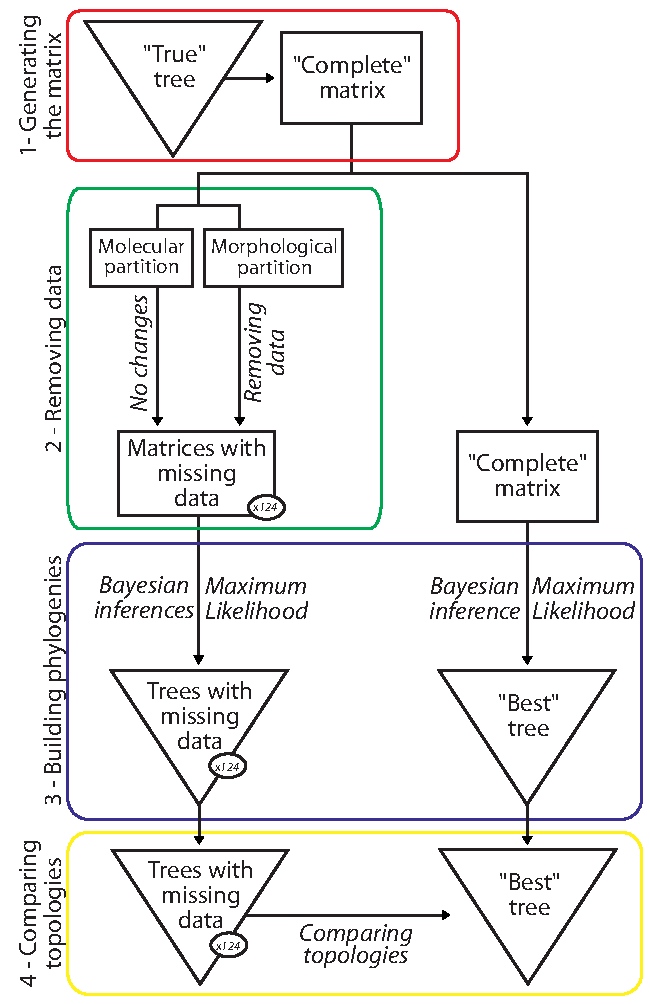
\includegraphics[keepaspectratio=true]{Figures/TEM_Fig_outline.pdf}
\caption{Protocol outline. (1) We generated a random tree (hereafter called the "true" tree) to infer a matrix with no missing data (hereafter, the "complete" matrix). (2) We removed data fron the morphological partition of the "Complete" matrix resulting in 124 matrices with missing data. (3) We build Bayesian phylogenetic trees from each matrix. (4) We then compared the trees with missing data (from the matrices with missing data) to the tree with no missing data (hereafter, the "best" tree – infered from the "complete" matrix). We repeated step 1 to 4 50 times.}
\label{Fig_Outline}
\end{figure}


\subsection{Generating the matrix}
First we randomly generated a "true" tree of 50 taxa in R v3.0.2 \citep{R302} using the package diversitree v0.9-6 \citep{fitzjohndiversitree2012}. We generated the tree using a Birth Death process by sampling the values of the speciation events ($\lambda$) and extinction events ($\mu$) from a uniform distribution but maintaining $\lambda$ $>$ $\mu$ \citep{paradistime-dependent2011}. We implemented a rejection sampling algorithm to select only random trees with 25 living and 25 fossil taxa. We then added a species to the resulting Birth-Death tree as the outgroup of the tree. The mean branch length of the tree was used to separate the outgroup from the rest of the taxa and the branch length leading to the outgroup was set as the sum of the mean branch length and the longest root-to-tip length of the tree.

Next, we created a molecular and a morphological matrix from the "true" tree. The molecular matrix was infered from the "true" tree using the package phyclust v0.1-14 \citep{chen2011}. The matrix was made of 1000 characters sites for 51 taxa and generated using the seqgen algorithm \citep{ ranbaut1997seqgen}. We used the HKY model \citep{HKY85} with a random base frequencies and with the transition/transversion rate of 2 \citep{douadycomparison2003} as parameters for generating the matrix. The substitution rates were distributed following a gamma distribution with an alpha ($\alpha$) shape of 0.5 \citep{yangamong-site1996}. We chose a low value of $\alpha$ to lower the number of sites with high substitution rates, thus avoiding too much homoplasy and a decrease in phylogenetic signal. These parameters were selected to generate data with no special assumption about how the characters evolved as well as to reduce the computational time required if these parameters were estimated rather than defined (65 CPU years).

We infered the morphological matrix using the ape package v3.0-8 \citep{paradisape:2004} to generate a matrix of 100 character sites for 51 taxa. We assigned the number of character states (either 2 or 3) for each morphological character by sampling with a probability of 0.85 for two states characters and 0.15 for three state characters. These probabilities were selected using the overall distribution of characters states extracted from 100 published empirical morphological matrices (See supplementaries). %link missing
We then ran an independent discrete character simulation for each character with the randomly selected number of states (2 or 3) and assuming an equal rate of change (i.e. evolutionary rate) from one character state to an other. This method allows us to have only two parameters per character i.e. the number of states and the evolutionary rate. For each character, the evolutionary rate was sampled from a gamma distribution with $\alpha$ = 0.5.  All the molecular information for fossil taxa was replaced by missing data ("?"). Finally, we combined the morphological and molecular matrices obtained from the "true" tree. Hereafter we call this the "complete" matrix, i.e. the matrix with no missing data except for the molecular data of the fossil taxa.

\subsection{Removing data}
Once we obtained the "complete" matrix we modified it to get a set of matrices with missing data. We randomly replaced data with “?” in the morphological part of the matrices according to the following parameters (Fig. ~\ref{Fig_RemoveData}):

\begin{enumerate}
\item{The proportion of living taxa with no morphological data ($M_{L}$): 0\%, 10\%, 25\%, 50\% or 75\%.}
This parameter illustrates the number of living taxa that are present in the molecular part of the matrix but not in the morphological one. Because of the increasing facility to sequence DNA for living species, the number of living species with molecular data is highly superior the the number of species with molecular and morphological data.
\item{The proportion of missing morphological data across all fossil taxa ($M_{F}$): 0\%, 10\%, 25\%, 50\% or 75\%.}
This parameter illustrates the quality of the fossil record. 
\item{The proportion of missing morphological characters across all taxa (living and fossil - $M_{C}$): 0\%, 10\%, 25\%, 50\% or 75\%. }
This parameter illustrates the number of available morphological characters for both living and fossil taxa.
\end{enumerate}

\begin{figure}
\centering
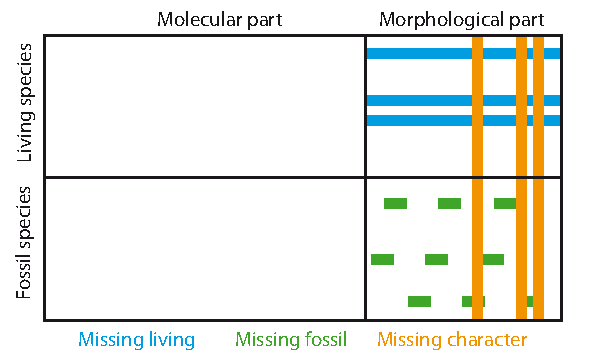
\includegraphics[keepaspectratio=true]{Figures/TEM_Fig_missingData.pdf}
\caption{Data removal protocol: Missing living - The proportion of living taxa with no morphological data ($M_{L}$); Missing fossil - The proportion of missing morphological data across all fossil taxa ($M_{F}$); Missing character - The proportion of missing morphological characters across all taxa (living and fossil) ($M_{C}$).}
\label{Fig_RemoveData}
\end{figure}

In practice, each parameter represent a way of removing data in the morphological part of the matrix: $M_{L}$ removes a proportion of rows from the living taxa; $M_{F}$ removes a proportion of cells from the fossil taxa; and $M_{C}$ removes a proportion of columns across both living and fossil taxa. Note that $M_{L}$ is different to $M_{F}$ not only because of the region of the supermatrix affected: for $M_{L}$, all the morphological data of a proportion of the living taxa is removed (i.e. removing rows), as for $M_{F}$, a proportion of data is removed across the whole of the morphological matrix for fossil taxa (i.e. removing cells).

We tested all parameters combinations resulting in 125 ($5^3$) matrices. Because some parameter combinations introduce a lot of missing (e.g. $M_L$=75\%, $M_F$=75\% and $M_C$=75\%), some matrices contained fossil taxa without any data at all. When this occurred we repeated the random deletion of characters until every species had at least 5\% data.

\subsection{Building phylogenies}
From the resulting matrices we generated two types of trees, the "best" tree that is infered from the "complete" matrix and the trees with missing data infered from the 125 matrices with various amounts of missing data. The "true" tree was used to generate the "complete" matrix and reflects the "true" evolutionary history in our simulations. The "best" tree, on the other hand, is the best tree we can build using the state-of-the-art phylogenetic methods. In real world situations, the "true" tree is never available to us because we cannot know the true evolutionnary history of a clade (except in very rare circumstances, e.g. \citet{rozen2005}). Therefore, here we focus on comparing the trees infered from the matrices with missing data to the "best" tree, rather than the "true" tree, as the "best" tree is generally what biologists have to work with.

\subsubsection{Maximum Likelihood}
The "best" tree and the "missing-data" trees were infered using RAxML v7.0.4 \citep{stamatakisthe2008}. We used the GTR + $\Gamma_4$ model (\citet{tavare1986} – default GTRGAMMA in RAxML v7.04) as a generalisation of the HKY + $\Gamma_4$ model \citep{HKY85} for the molecular data. The GTR model can be seen as a generalisation of the HKY model (the 2 parameters from the HKY model are implicitly included in the 6 from GTR model - \citet{stamatakisa2008}). We used the fast bootstrap algorithm and performed 1000 bootstraps per tree inference to assess the topological support. %Mk model seems implemented (i.e. Aprils’s slideshare http://www.slideshare.net/wrightaprilm/evolution2013). But how? Default method for standard data type (i.e. non DNA/AA). Trevor: swapping algorithm? salanin 2003

\subsubsection{Bayesian}
The "best" tree and the "missing-data" trees were infered using MrBayes v3.2.2 \citep{Ronquist2012mrbayes}. We partitioned the data treating the molecular part as a non-codon DNA partition and the morphological part as a multi-state morphological partition. The molecular evolutionary history was infered using the HKY model with a transition/transversion ratio \citep{douadycomparison2003} of two and a gamma distribution for the rate variation with four distinct categories (HKY + $\Gamma_4$). For the morphological data, we used the Markov \textit{k} state model \citep{lewisa2001} wich is a generalisation of the JC69 model \citep{jc69} with \textit{k} $≥$ 2, assuming an equal state frequency and a unique overall substitution rate ($\mu$) following a gamma distribution of the rate variation with four distinct categories (M\textit{k} + $\Gamma_4$). We chose these models to be consistent with the parameters used to generate the "complete" matrix.

Each Bayesian tree was estimated using two runs of four chains each for a maximum of 50$\times$$1^6$ generations. We used the average standard deviation of split frequencies (ASDS) as a proxy to estimate the convergence of the chains and implemented a stop rule when the ASDS went below 0.01 \citep{Ronquist2012mrbayes}. The effective sample size (ESS) was also checked on a random subsample of runs in each simulation to check that ESS $>>$ 200 \citep{drummond2006ess}. For each run, we removed 25\% of the iterations as burnin. We used the following priors for each tree (see supplementaries): %link missing
\begin{enumerate}
\item
the "true" tree’s topology as a starting tree (with a starting value for each branch length of 1),
\item
an exponential prior on the shape of the gamma distribution of $\alpha$=0.5 for both partitions
\item
and a transition/transversion ratio prior of 2 sampled from a strong beta distribution ($\beta$(80,40)).
\end{enumerate}

We used these priors to speed up the Bayesian process. These priors biased the way the Bayesian process calculated the branch length by giving non-random starting points and boundaries for the parameters estimation process, however, we are focusing on the effect of missing data on the topology and not on the branch length. Even using these priors, it took 65 CPU years to build 50 sets of 125 Bayesian trees (8 core nodes 2.30GHz clock speed).

\subsection{Comparing topologies}
We compared the topology of the "missing-data" trees infered from the matrices with missing data to the "best" tree to measure the effect of the three parameters $M_{L}$, $M_{F}$ and $M_{C}$. Note that we only investigate differences in topology and not in branch length because the aim of this study is to look at the effect of missing data on the topology of trees infered from supermatrices with living and fossil species and molecular and morphological characters. To compare the topology of the resulting trees, we used two metrics to assess number of conserved taxa and clades position using respectively the Triple \citep{dobson1975triplets} and the Robison-Fould \citep{RF1981} distance. We normalised the two metrics using the Normalised Tree Similarity index \citep{Bogdanowicz2012} to generalise our results for any n number of taxa. The two metrics and the index are detailed below.

\subsubsection{Triple distance ($T_{x,y}$) \citep{dobson1975triplets}}
This metric measures the number of different subtrees of three clades between two given trees. Each triplet can be written as $I_{ijk}$=(\textit{ijk}). Where $I_{ijk}$ is equal to 0 if the the two triplets (\textit{ijk}) are the same in the two trees otherwise $I_{ijk}$ is equal to 1. For any rooted binary tree there are only three possible combinations per triplets: ((\textit{j},\textit{k}),\textit{i});, ((\textit{i},\textit{k}),\textit{j}); and ((\textit{i},\textit{j}),\textit{k}); \citep{johnson1998}. If the trees used are not fully binary, a fourth triplet combination is possible: (\textit{i},\textit{j},\textit{k});.One can calculate $S_n$, the triplet distance between two trees as:
\begin{equation}
S_n = \sum_{ijk} I_{ijk}
\end{equation}
Where:
\begin{equation}
\sum_{ijk} = \binom{n}{4} = \frac{n!}{4!(n-4)!}
\end{equation}
And where \textit{n} is the number of taxa in both trees (modified from \citet{critchlowthe1996}). If $S_n$=0, the trees are the same (i.e. no taxa as been displaced). When $S_n$ = $\binom{n}{4}$, the trees are the most different possible (i.e. every taxa as been displaced). This metric therefore illustrates the amount of displaxed taxa but is less sensitive to the placement of individual taxa and to taxa of highly uncertain placement (e.g. fossil taxa) than the Robinson-Foulds distance \citep{critchlowthe1996,johnson1998,wiensmissing2003} and can therefore be used as a proxy to estimate the robustness of the tree to flying taxa (see supplementaries). %link missing

\subsubsection{Robinson-Fould distance (\textit{RF}) \citep{RF1981}}
This metric measures the number of shared clades among two trees and therefore illustrates the number of exactly conserved groups among the trees. The Robison-Fould distance (also called path difference) between two trees reflects the distance between the distributions of the tips among clades in the two trees \citep{RF1981} and can be expressed as following:
\begin{equation}
RF_{x,y} = N_{x} + N_{y} - 2C_{x,y}
\end{equation}
Where $C_{x,y}$ is the number of clades in common in the two trees. The minimal value of \textit{C} is 1 if the two trees have the same \textit{n} taxa; the maximal value in \textit{C=n-2}. This metric is more sensitive to taxa displacement than the triple metric (if one taxa gets out of a clade, then the clades are no longer considered as similar - \citet{critchlowthe1996,johnson1998,wiensmissing2003}) and therefore a low value will show a good clade conservation between two trees and a high value will show a bad recovery of common clades (see supplementaries). %link missing

\subsubsection{Normalised Tree Similarity \textit{NTS} \citep{Bogdanowicz2012}}
For any tree with \textit{n} taxa compared using a tree distance metric \textit{m}, $NTS_m$ represents the similarity score between the two trees given the expected distance between two random Yule trees with \textit{n} taxa. Let $\bar{d}_{m,n}$\textit{(rand)} be the average distance between two random Yule trees with \textit{n} taxa and $d_{m,n}$\textit{(x,y)} the distance between the two trees \textit{x} and \textit{y} containing each \textit{n} taxa, then:
\begin{equation}
NTS_{m,n}(x,y)=\frac{\bar{d}_{m,n}(rand) - d_{m,n}(x,y)} {\bar{d}_{m,n}(rand)}
\end{equation}
\textit{NTS} ranges from 1 to -$\infty$. For any \textit{m},\textit{n} when \textit{NTS}=1, the trees are the same; when \textit{NTS}=0 the trees are not more different than expected by chance; when \textit{NTS}$<$0, the trees are more different than expected by chance (see supplementaries). %link missing

$\newline$

We compared the "missing-data" tree to the "True" and the "Best" tree for each chain. For the Maximum Likelihood trees we performed pairwise comparisons between the "True" and "Best" tree and \textit{Y} (where \textit{Y} is one of the 125 trees resulting from the 125 super matrices including various amount of missing data) for both the Robinson-Fould and the Triple metric. We calculated the metrics using the TreeCmp java script \citep{Bogdanowicz2012}. For each metric, we normalized the value using the Normalised Tree Similarity scaled with the mean value of 1000 pairwise random tree comparison for the same metric and the same number of taxa \textit{n}=51 (see supplementaries). %link missing
We rand the comparison for the 50 trees of each chain having the same combination of parameters values $M_L$, $M_F$ and $M_C$. We calculated the mode and the 50, 75 and 95 confidence intervals for each comparison of 50 trees using the hdrcde R package (v3.1 – \citet{hdrcde}). For the Bayesian trees, we used the exact same approach described above but instead of comparing the "True" or "Best" tree to the tree \textit{Y}, we compared 1000 trees from the "True" or "Best" tree posterior distribution to 1000 trees from the tree \textit{Y} posterior distribution resulting in 1000 pairwise comparison of the "True" or "Best" tree to the tree \textit{Y} for each 125 trees (see supplementaries - Fig. ~\ref{Fig_Compare}). %link missing

\begin{figure}
\centering
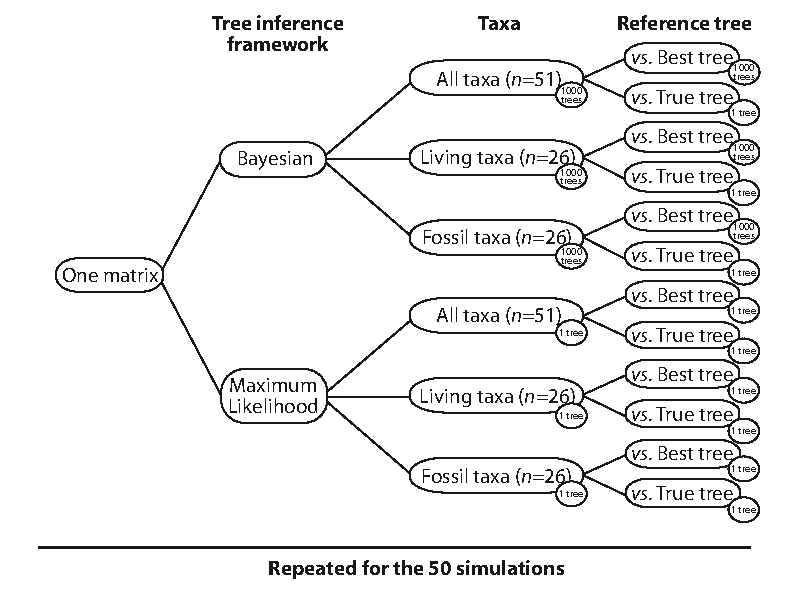
\includegraphics[keepaspectratio=true]{Figures/TEM_Fig_TreeCmp3.pdf}
\caption{Tree comparison protocol. From each of the 125 parameters combination ($M_L$, $M_F$ and $M_C$), we infered a tree in Baysian or Maximum likelihood framework. We then compared this tree with or without fossil/living taxa to the "best/true" tree. In the Bayesian framework, 1000 trees from the posterior ditribution where used for each comparison.}
\label{Fig_Compare}
\end{figure}

\subsection{Empirical data}
We also compared the results obtained from simulated data by using \citet{ronquista2012} empirical data. The supermatrix contains 67 living species plus one outgroup and 45 fossil species of Hymenopteras with 5097 molecular characters and 354 morphological characters. From the 68 living species used in the supermatrix, only 66 had molecular data %missing???
, we therefore treated these 66 taxa as "living" taxa and all the other 47 as "fossil" taxa. We treated the matrix in the exact same way as described in step 2 and 3 resulting in 125 supermatrices with various amount of missing data and the same number of Maximum Likelihood and Bayesian trees. We used the same settings as for the simulated data in the Maximum Likelihood framework. For the Bayesian inferences however, we didn’t used any priors except that we provided a starting tree with the topology of the 68 living species (topology with the highest posterior probability from non-clock analysis - \citet{ronquista2012}). Contrary to \citet{ronquista2012} analysis, we didn’t performed any clock analysis since we were only interested in the topology of the infered tree and not the branch length.

\section{Results}
%Baysian inference doesn’t recover the topology, whatever the amount of data
%Bayesian inference with or without the fossil/living doesn’t recover the topology, whatever the amount of data
%Likelihood inference recovers the topology depending on the amount of data
%Likelihood with only living recovers the topology really well
%Likelihood with only fossil??

\section{Discussion}


\section{Supplementaries}
\label{supplementaries}
blabla
%BIBLIOGRAPHY
 % The \cite command functions as follows:
 %   \citet{key} ==>>                Jones et al. (1990)
 %   \citet*{key} ==>>               Jones, Baker, and Smith (1990)
 %   \citep{key} ==>>                (Jones et al., 1990)
 %   \citep*{key} ==>>               (Jones, Baker, and Smith, 1990)
 %   \citep[chap. 2]{key} ==>>       (Jones et al., 1990, chap. 2)
 %   \citep[e.g.][]{key} ==>>        (e.g. Jones et al., 1990)
 %   \citep[e.g.][p. 32]{key} ==>>   (e.g. Jones et al., p. 32)
 %   \citeauthor{key} ==>>           Jones et al.
 %   \citeauthor*{key} ==>>          Jones, Baker, and Smith
 %   \citeyear{key} ==>>             1990

\bibliographystyle{sysbio} %don't write the suffix
\bibliography{References} %don't write the suffix

%END
\end{document}